\section{Einleitung}

Heutzutage ist es üblich, dass Präsentationen durch Teilnehmer bewertet werden. Dieses Feedback wird entweder durch Fragebögen oder mit Hilfe von browserbasierten Anwendungen wie z.B. \emph{joind.in}\footnote{\url{http://joind.in/}} nach einer Präsentation erfasst. Hierbei bewerten die Teilnehmer die Präsentation sowohl im Hinblick auf die didaktische Aufbereitung als auch auf "`weiche"' Faktoren wie z.B. das persönliche Auftreten des Präsentierenden. Diese Bewertung spiegelt immer den subjektiven Eindruck der Teilnehmer über den Verlauf der gesamten Präsentation wieder -- eine individuelle Bewertung einzelner Folien ist dabei nicht möglich. Um bessere und genauere Bewertungen zu erhalten, müssten diese idealerweise schon im Laufe einer Präsentation abgegeben werden können. Es fehlt also ein direkter, verzögerungsfreier Kanal um Bewertungen einer Präsentation durch deren Teilnehmer zu erfassen.

Feedback muss dabei nicht auf die Bewertung einer Veranstaltung beschränkt sein. Eine interaktive Beteiligung durchbricht den üblichen Ablauf von Präsentation, bei denen eine Person vorträgt und alle anderen passiv zuhören. So kann man eine bessere Aufnahme des Themas bei den Teilnehmern erreichen. Beispiel hierfür sind Aufgaben, die von den Teilnehmern durch Auswählen einer Antwort gelöst werden, und bei denen anschließend die Ergebnisse aller Teilnehmer gemittelt dargestellt werden. Diese Art von Interaktion dient zur schnellen Kontrolle des Wissensstandes für den einzelnen, liefert aber auch dem Lehrenden einen schnellen und direkten Überblick über den Leistungsstand der Teilnehmer. Hierfür existieren schon Systeme wie \emph{QuizDom}\footnote{\url{http://www.qwizdom.com/}}, bei denen Klassenraum-Ausstattungen aber leicht mehrere tausend Euro kosten\footnote{\url{http://www.dreamav.co.uk/qwizdom_q4.html}}. Mit diesen Geräten können die Teilnehmer, nachdem die Geräte an jeden Einzelnen ausgeteilt wurden, Fragen mithilfe der Tastatur auf den Geräten beantworten, die dann unmittelbar ausgewertet werden können. Ein direkter Rückkanal zum Teilnehmer existiert aber hierbei nicht.

\section{Gruppenbefragung}
\label{l:gruppenbefragung}

Gerade bei jüngeren Personen und im Business-Umfeld sind SmartPhones inzwischen sehr weit verbreitet -- \emph{GroupMood} schafft für Teilnehmer die Möglichkeit, Veranstaltungen jeder Art auf dem eigenen mobilen Endgerät direkt zu bewerten. Dadurch sind die Teilnehmer in der Lage direkt in jeder Veranstaltung individuelles Feedback zu geben, dass dann unmittelbar ausgewertet und analysiert werden kann. 

\begin{table}[htb]
\begin{center}
\begin{tabular}{l c c}
Kriterium & Einzelne Folien & gesamte Präsentation \\
\hline
Inhaltliches Verständnis & \checkmark & \checkmark \\
Geschwindigkeit des Vortrages & --- & \checkmark \\
Verständlichkeit des Sprechers & --- & \checkmark \\
Bewertung & \checkmark & \checkmark \\
Kommentare & \checkmark & --- \\
\end{tabular}
\caption{Bewertungsmöglichkeiten in einer Präsentation}
\label{table:meetingratings}
\end{center}
\end{table}

Um die Bewertung von Präsentationen mit der App zu ermöglichen, erstellt der Vortragende vorab einen Foliensatz und fügt an den geeigneten Stellen Umfragen ein. Der Foliensatz wird auf die Geräte aller Teilnehmer verteilt. Die Teilnehmer können anschließend innerhalb der Anwendung zwischen den einzelnen Folien navigieren und die zugeordneten Umfragen beantworten. So ist es für die Teilnehmer auch möglich, die einzelnen Folien der Präsentation zu bewerten. Mögliche Kriterien, die von den Teilnehmer mit Hilfe der Umfragen die bewertet werden können, sind in Tabelle~\ref{table:meetingratings} aufgeführt. Am Ende der Präsentation erhalten die Teilnehmer eine Ansicht in der sie eine Gesamtbewertung der Präsentation vornehmen können.

\begin{figure}[htb]
\begin{center}
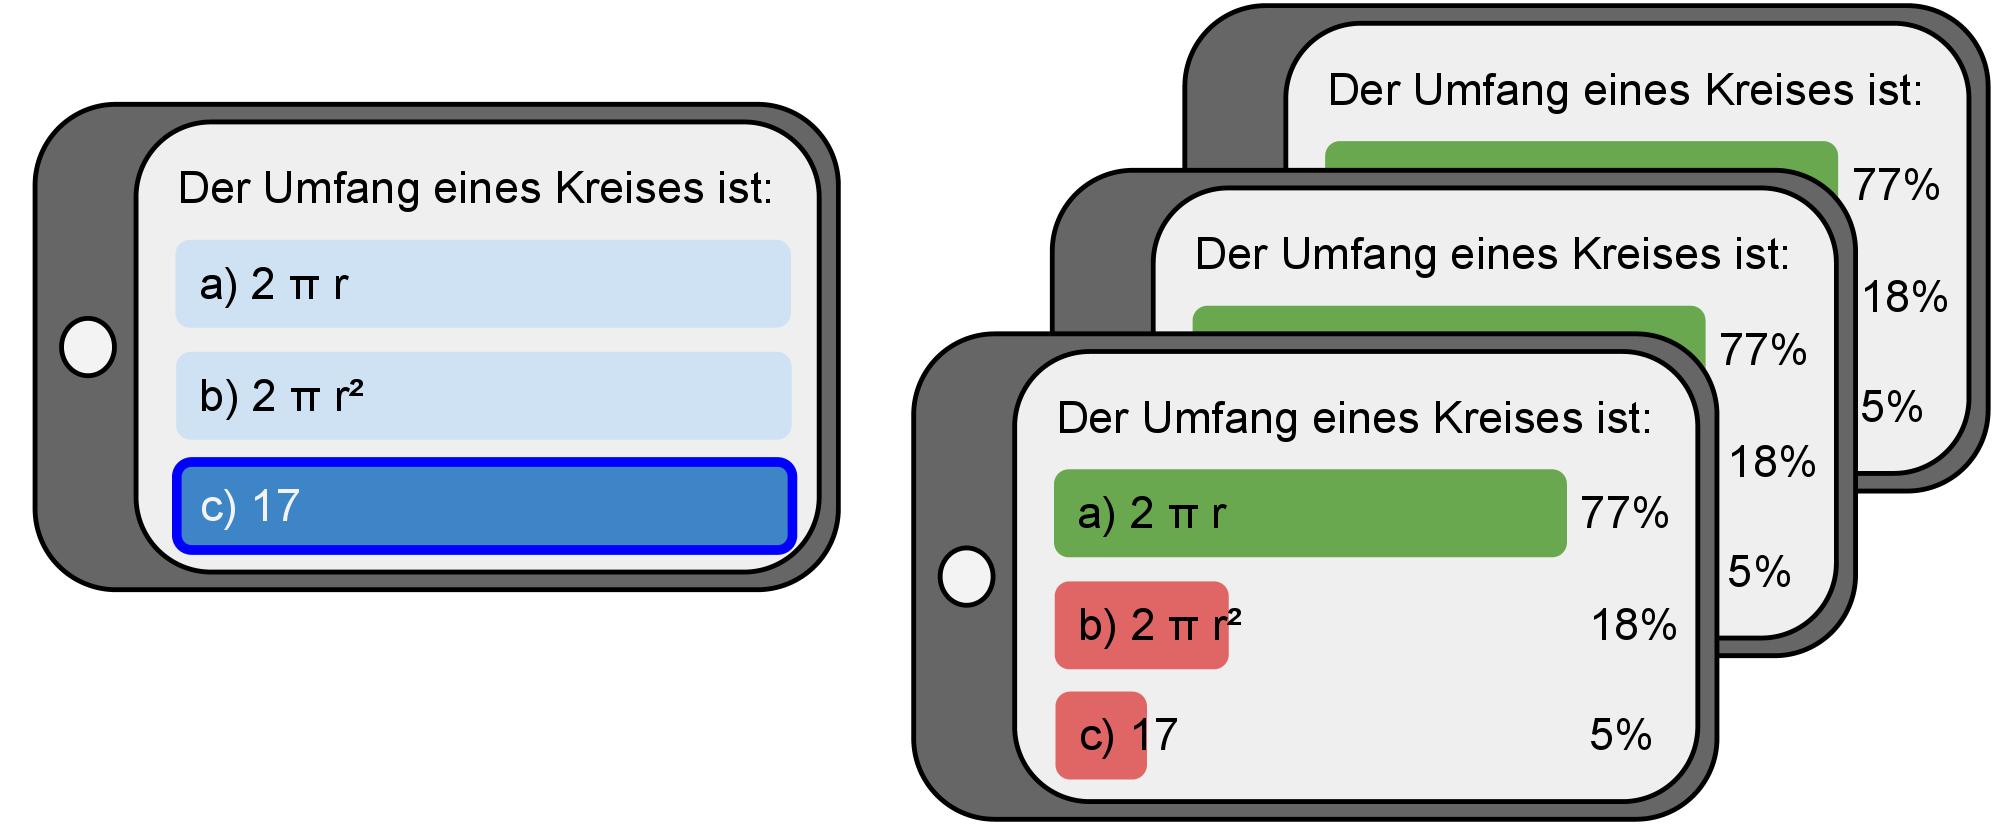
\includegraphics[width=0.75\textwidth]{media/Umfrage.png}
\end{center}
\caption{Eine einfache Umfrage}
\label{f:umfrage}
\end{figure}

Abbildung~\ref{f:umfrage} zeigt schematisch die Darstellung einer Umfrage. In der Anwendung sind insgesamt drei Arten von Umfragen möglich: bei \emph{Einfach-Auswahl-Fragen} muss genau eine Antwort ausgewählt werden, bei \emph{Mehrfach-Auswahl-Fragen} muss eine oder mehrere Antworten ausgewählt werden und bei \emph{Wert-Eingaben} wird als Antwort eine Zahl erwartet, wobei der Fragesteller den möglichen Wertebereich einschränken kann. Mit diesen Frage-Typen ist es möglich beliebige andere Gruppenbefragungen durchzuführen. Abbildung~\ref{f:fotoabstimmung} zeigt schematisch den Einsatz der Anwendung in einer Foto-Abstimmung. Die Teilnehmer der Gruppe können mit ihren Mobilgeräten Fotos machen oder vom Gerät auswählen und zur Abstimmung stellen. Die Fotos werden in der Gruppe verteilt und bei der Abstimmung kann jeder Teilnehmer alle Fotos auf seinem Gerät betrachten und bewerten.

\begin{figure}[htb]
\begin{center}
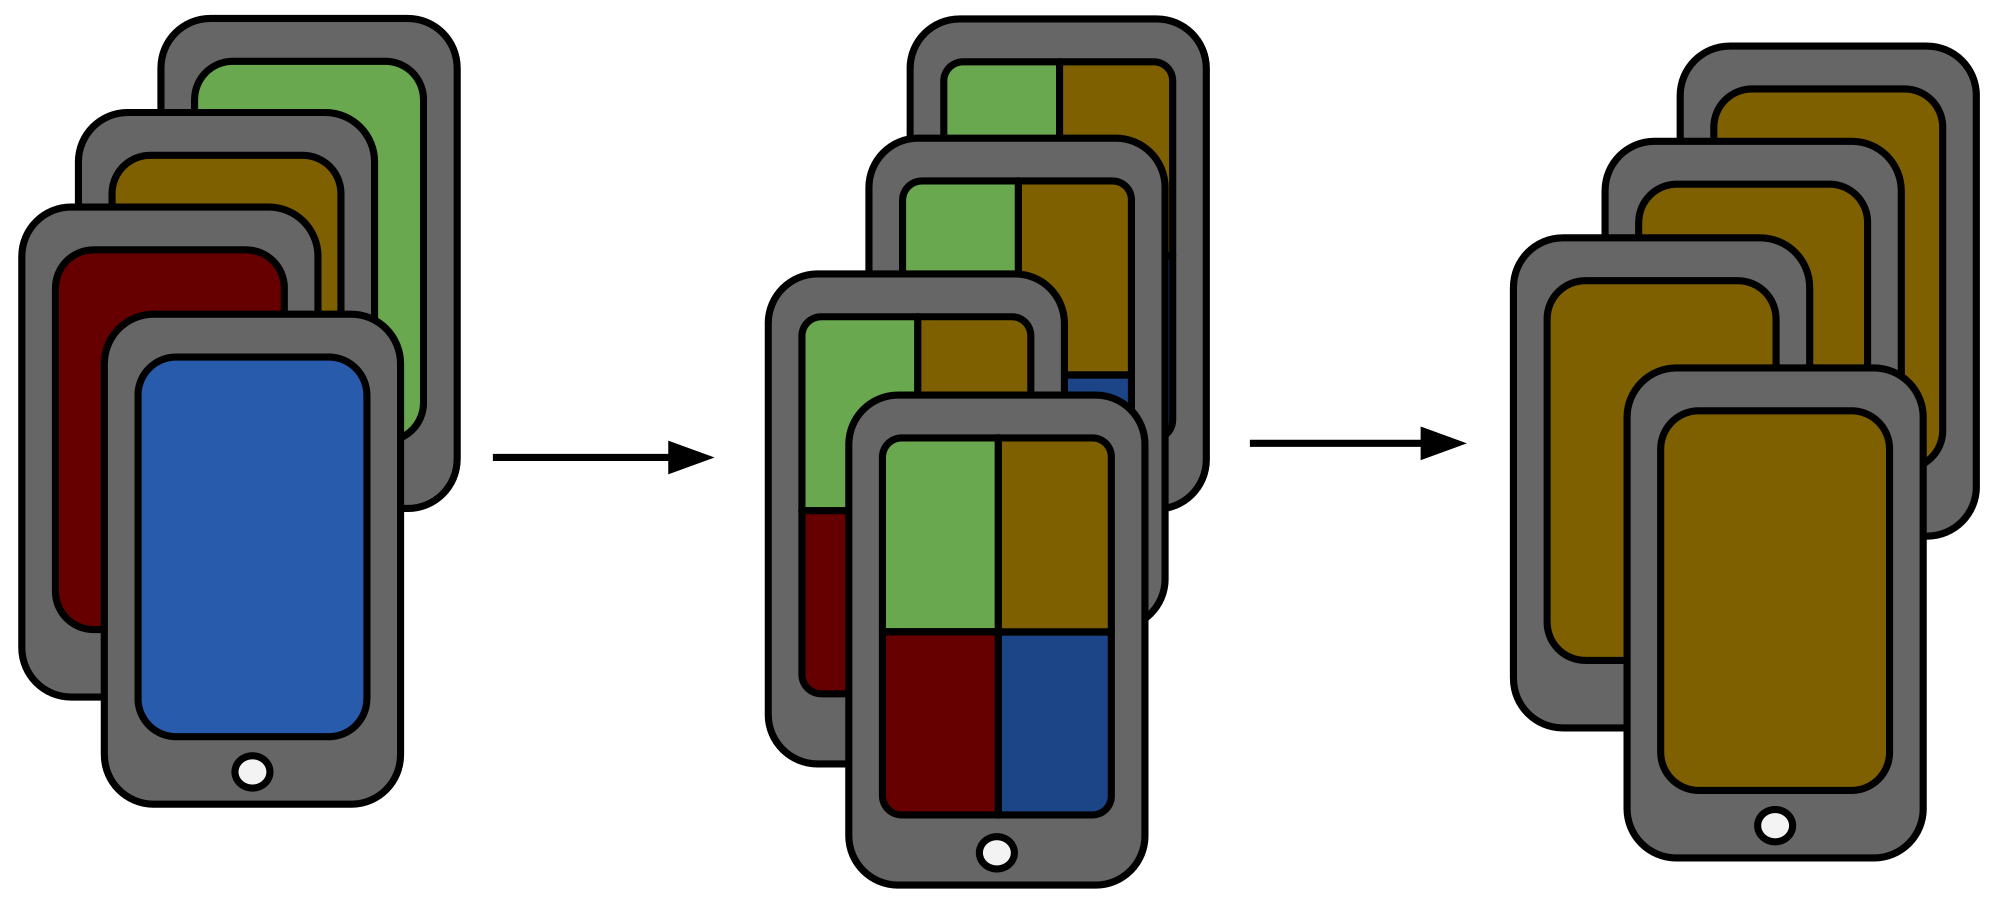
\includegraphics[width=0.75\textwidth]{media/Fotoabstimmung.png}
\end{center}
\caption{Foto-Abstimmung}
\label{f:fotoabstimmung} 
\end{figure}
